\documentclass[11pt]{article}
\usepackage[margin=1in]{geometry}
\usepackage{amsmath}
\usepackage{amssymb}
\usepackage{hyperref}
\usepackage{xcolor}
\usepackage{booktabs}
\usepackage{tikz}
\usetikzlibrary{arrows.meta,positioning,shapes,fit,calc}
\usepackage{pgfplots}
\pgfplotsset{compat=1.18}

\title{Context-Aware FinCommerce Pipeline (End-to-End Report)}
\author{}
\date{January 22, 2026}

\begin{document}
\maketitle

\section*{Overview}
This report documents the full end-to-end Context-Aware FinCommerce pipeline implemented in this workspace. It covers:
\begin{itemize}
  \item Data preparation from Amazon CSV into JSON payloads.
  \item Qdrant collection schema creation (4 collections + payload indexes).
  \item Synthetic but \emph{correlated} user profiles, financial context, and interaction history.
  \item Embedding generation and batched upserts to Qdrant Cloud with retry/backoff.
  \item Semantic search and a personalized reranker (affordability + preferences).
\end{itemize}

\paragraph{Code map (scripts).}
\begin{itemize}
  \item \texttt{data/prepare\_data.py}: CSV \textrightarrow JSON with semantic category assignment + brand extraction.
  \item \texttt{qdrant\_setup.py}: creates/recreates collections and payload indexes.
  \item \texttt{generate\_and\_insert\_data.py}: embeds and inserts products, users, financials, interactions.
  \item \texttt{search\_pipeline.py}: query embedding, Qdrant search, rerank, and output.
\end{itemize}

\paragraph{Environment variables.}
The pipeline expects \texttt{QDRANT\_URL} and \texttt{QDRANT\_API\_KEY} to be set (e.g., via \texttt{.env}).

\section*{Pipeline Diagram (What Happens End-to-End)}
\begin{center}
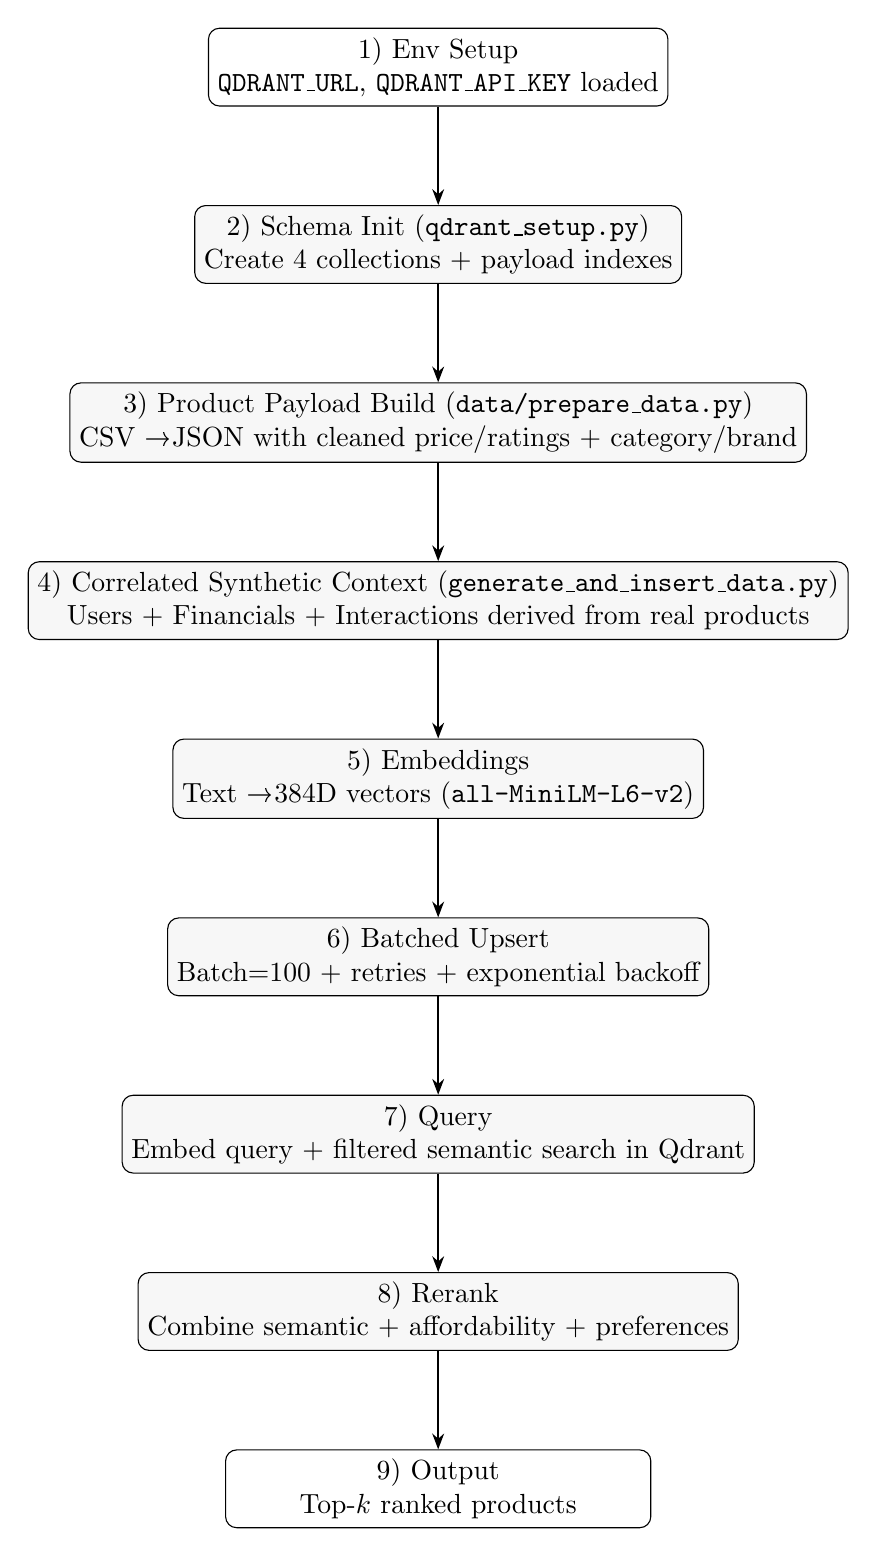
\begin{tikzpicture}[
  node distance=1.25cm,
  box/.style={rectangle, rounded corners, draw=black, align=center, minimum width=5.4cm, minimum height=0.95cm},
  sbox/.style={rectangle, rounded corners, draw=black, align=center, minimum width=5.4cm, minimum height=0.78cm, fill=black!3},
  arrow/.style={-{Stealth[length=2mm]}, thick}
]

\node[box] (env) {1) Env Setup\\\texttt{QDRANT\_URL}, \texttt{QDRANT\_API\_KEY} loaded};
\node[sbox, below=of env] (schema) {2) Schema Init (\texttt{qdrant\_setup.py})\\Create 4 collections + payload indexes};
\node[sbox, below=of schema] (payload) {3) Product Payload Build (\texttt{data/prepare\_data.py})\\CSV \textrightarrow JSON with cleaned price/ratings + category/brand};
\node[sbox, below=of payload] (gen) {4) Correlated Synthetic Context (\texttt{generate\_and\_insert\_data.py})\\Users + Financials + Interactions derived from real products};
\node[sbox, below=of gen] (embed) {5) Embeddings\\Text \textrightarrow 384D vectors (\texttt{all-MiniLM-L6-v2})};
\node[sbox, below=of embed] (upsert) {6) Batched Upsert\\Batch=100 + retries + exponential backoff};
\node[sbox, below=of upsert] (search) {7) Query\\Embed query + filtered semantic search in Qdrant};
\node[sbox, below=of search] (rerank) {8) Rerank\\Combine semantic + affordability + preferences};
\node[box, below=of rerank] (output) {9) Output\\Top-$k$ ranked products};

\draw[arrow] (env) -- (schema);
\draw[arrow] (schema) -- (payload);
\draw[arrow] (payload) -- (gen);
\draw[arrow] (gen) -- (embed);
\draw[arrow] (embed) -- (upsert);
\draw[arrow] (upsert) -- (search);
\draw[arrow] (search) -- (rerank);
\draw[arrow] (rerank) -- (output);

\end{tikzpicture}
\end{center}

\section*{Collections, Vectors, and Payloads}
The pipeline stores data in 4 Qdrant collections. Three collections use 384D text embeddings. Financial context uses 256D vectors (a numeric/placeholder representation).

\begin{center}
\begin{tabular}{llll}
\toprule
\textbf{Collection} & \textbf{Vector Dim} & \textbf{Distance} & \textbf{Key Payload Fields}\\
\midrule
\texttt{products\_multimodal} & 384 & Cosine & product\_id, name, category, brand, price, in\_stock, region\\
\texttt{user\_profiles} & 384 & Cosine & user\_id, name, location, risk\_tolerance, preferred\_categories, preferred\_brands\\
\texttt{financial\_contexts} & 256 & Cosine & user\_id, available\_balance, credit\_limit, current\_debt, eligible\_installments\\
\texttt{interaction\_memory} & 384 & Cosine & user\_id, query, clicked\_product\_id, purchased\\
\bottomrule
\end{tabular}
\end{center}

\subsection*{Schema Creation (\texttt{qdrant\_setup.py})}
The schema script recreates collections and then creates payload indexes. Indexes matter because they make filters (e.g., \texttt{price}, \texttt{in\_stock}) efficient and reliable.

\paragraph{Why payload indexes?}
Search is a combination of vector similarity and structured filters. Payload indexes allow Qdrant to efficiently apply constraints like:
\begin{itemize}
  \item \texttt{price <= max\_price}
  \item \texttt{in\_stock = true}
  \item \texttt{category} / \texttt{brand} matching
\end{itemize}

\section*{Step 1: Data Preparation (CSV \textrightarrow JSON)}
\subsection*{Input}
The primary product source is an Amazon export CSV (e.g., \texttt{data/All Electronics.csv}) with fields such as:
\texttt{name}, \texttt{image}, \texttt{ratings}, \texttt{no\_of\_ratings}, \texttt{discount\_price}, \texttt{actual\_price}.

\subsection*{Cleaning and normalization (\texttt{data/prepare\_data.py})}
Key transformations:
\begin{itemize}
  \item Price parsing: remove currency symbols/commas and convert to numeric.
  \item Rating count parsing: \texttt{"113,956"} \textrightarrow \texttt{113956}.
  \item De-duplication: drop repeated products by normalized name.
  \item Fill additional fields used downstream: \texttt{region}, \texttt{in\_stock}.
\end{itemize}

\subsection*{Semantic category assignment}
Because the CSV's top-level category is often generic, categories are inferred from the product title using embeddings.

Let $e \in \mathbb{R}^{384}$ be the normalized embedding of the product name, and let $c_k \in \mathbb{R}^{384}$ be the normalized embedding of category description $k$.
The chosen category is:
\[
\hat{k} = \arg\max_k \; e^\top c_k
\]

\subsection*{Brand extraction}
Brand is extracted from the product title using lightweight heuristics (e.g., first meaningful token) to support preference matching.

\section*{Step 2: Synthetic Context Generation (Correlated, Not Random)}
\subsection*{Why correlation matters}
If user profiles and interactions are generated independently from products, personalization becomes meaningless. This pipeline derives user preferences and financial context from the actual product distribution so that:
\begin{itemize}
  \item Users tend to prefer categories/brands that exist in the catalog.
  \item Interactions (click/purchase) are biased toward preferred categories.
  \item Financial context (balances/limits) is scaled relative to observed product prices.
\end{itemize}

\subsection*{Generated entities (\texttt{generate\_and\_insert\_data.py})}
\begin{itemize}
  \item \textbf{Products}: loaded from JSON, embedded, inserted.
  \item \textbf{Users}: preferences sampled from product categories/brands.
  \item \textbf{Financial contexts}: derived per user using price statistics from preferred categories.
  \item \textbf{Interactions}: queries and clicks generated, biased by user preferences.
\end{itemize}

\section*{Step 3: Embeddings (Text \textrightarrow Vectors)}
The system uses SentenceTransformers \texttt{all-MiniLM-L6-v2}:
\begin{itemize}
  \item 384-dimensional embeddings for product text, user profile text, and interaction text.
  \item GPU acceleration when available (CUDA).
\end{itemize}

\section*{Step 4: Batched Upserts + Retry/Backoff (Qdrant Cloud Stability)}
Large single upserts can time out on hosted Qdrant. The solution used across products/users/financials/interactions is:
\begin{itemize}
  \item Batch size $B=100$ points.
  \item Up to $R=3$ retries per batch.
  \item Exponential backoff between retries (e.g., 1s, 2s, 4s).
\end{itemize}

\subsection*{Batching diagram}
\begin{center}
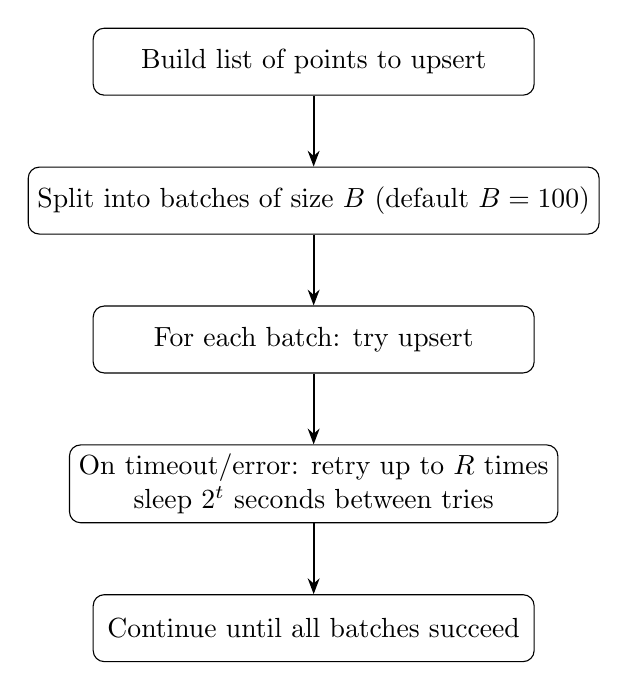
\begin{tikzpicture}[
  node distance=0.9cm,
  box/.style={rectangle, rounded corners, draw=black, align=center, minimum width=5.6cm, minimum height=0.85cm},
  arrow/.style={-{Stealth[length=2mm]}, thick}
]
\node[box] (build) {Build list of points to upsert};
\node[box, below=of build] (split) {Split into batches of size $B$ (default $B=100$)};
\node[box, below=of split] (try) {For each batch: try upsert};
\node[box, below=of try] (retry) {On timeout/error: retry up to $R$ times\\sleep $2^t$ seconds between tries};
\node[box, below=of retry] (done) {Continue until all batches succeed};

\draw[arrow] (build) -- (split);
\draw[arrow] (split) -- (try);
\draw[arrow] (try) -- (retry);
\draw[arrow] (retry) -- (done);
\end{tikzpicture}
\end{center}

\section*{Step 5: Search Pipeline (Semantic Search + Personalized Rerank)}
\subsection*{Semantic search (\texttt{search\_pipeline.py})}
Given a query string, the pipeline:
\begin{enumerate}
  \item Embeds the query to a 384D vector.
  \item Queries \texttt{products\_multimodal} by vector similarity.
  \item Applies structured filters when enabled (e.g., max price, in stock).
\end{enumerate}

\subsection*{User context retrieval}
The pipeline retrieves the user profile and financial context using \texttt{user\_id} and merges them into a single context object used for reranking.

\section*{Reranking Model}
The reranker combines three signals:
\begin{itemize}
  \item Semantic similarity score from Qdrant (higher is better).
  \item Affordability score based on user available balance vs product price.
  \item Preference score based on category/brand matches.
\end{itemize}

\subsection*{Core scoring formula}
\[
\text{final\_score} = 0.45\, s_{\text{semantic}} + 0.35\, s_{\text{afford}} + 0.20\, s_{\text{pref}}
\]

\[
 s_{\text{afford}} = \begin{cases}
0, & \text{if } \text{available\_balance} \le 0 \\
\max\left(0, 1 - \frac{\text{price}}{\text{available\_balance}}\right), & \text{otherwise}
\end{cases}
\]

\[
 s_{\text{pref}} = \max\left(\mathbb{1}[\text{category} \in \text{preferred\_categories}],\ \mathbb{1}[\text{brand} \in \text{preferred\_brands}]\right)
\]

\section*{Graphs for Better Understanding}
\subsection*{Score weights (bar chart)}
\begin{center}
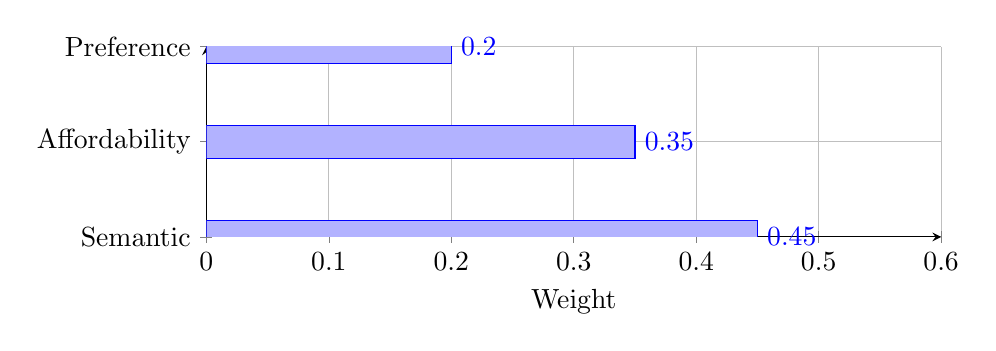
\begin{tikzpicture}
\begin{axis}[
  xbar,
  width=0.9\textwidth,
  height=4cm,
  xmin=0,
  xmax=0.6,
  xlabel={Weight},
  symbolic y coords={Semantic,Affordability,Preference},
  ytick=data,
  bar width=12pt,
  nodes near coords,
  nodes near coords align={horizontal},
  axis x line=bottom,
  axis y line=left,
  grid=major,
]
\addplot coordinates {(0.45,Semantic) (0.35,Affordability) (0.20,Preference)};
\end{axis}
\end{tikzpicture}
\end{center}

\subsection*{How the code fits together (script-level sequence)}
\begin{center}
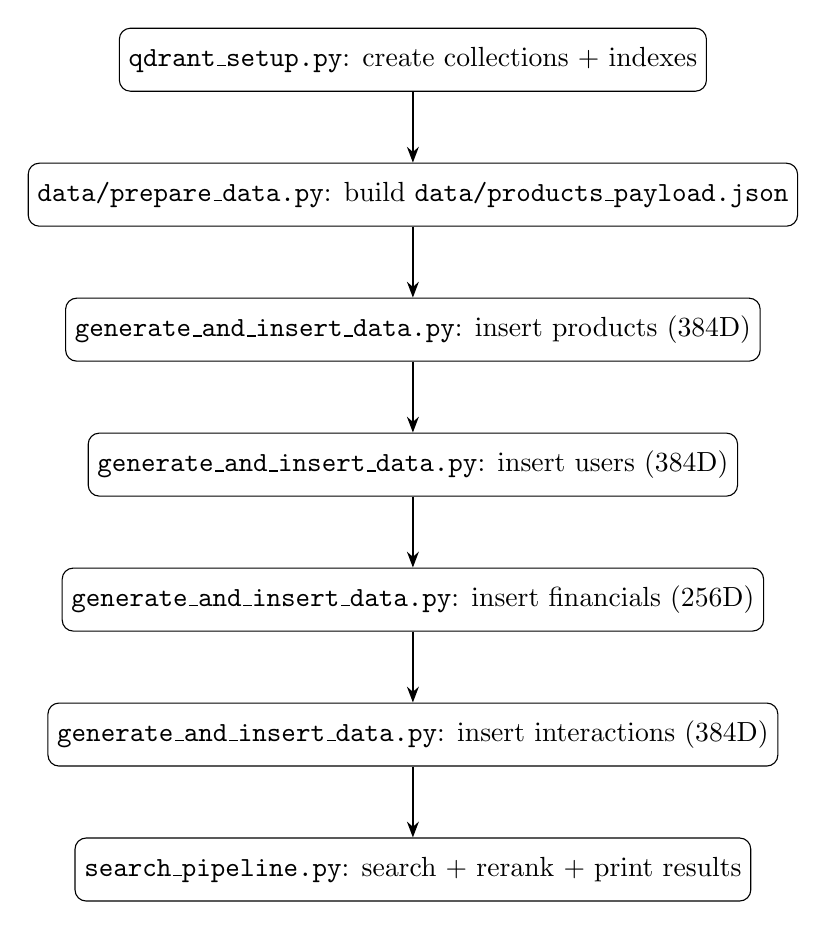
\begin{tikzpicture}[
  node distance=0.9cm,
  box/.style={rectangle, rounded corners, draw=black, align=center, minimum width=6.0cm, minimum height=0.8cm},
  arrow/.style={-{Stealth[length=2mm]}, thick}
]
\node[box] (s1) {\texttt{qdrant\_setup.py}: create collections + indexes};
\node[box, below=of s1] (s2) {\texttt{data/prepare\_data.py}: build \texttt{data/products\_payload.json}};
\node[box, below=of s2] (s3) {\texttt{generate\_and\_insert\_data.py}: insert products (384D)};
\node[box, below=of s3] (s4) {\texttt{generate\_and\_insert\_data.py}: insert users (384D)};
\node[box, below=of s4] (s5) {\texttt{generate\_and\_insert\_data.py}: insert financials (256D)};
\node[box, below=of s5] (s6) {\texttt{generate\_and\_insert\_data.py}: insert interactions (384D)};
\node[box, below=of s6] (s7) {\texttt{search\_pipeline.py}: search + rerank + print results};

\draw[arrow] (s1) -- (s2);
\draw[arrow] (s2) -- (s3);
\draw[arrow] (s3) -- (s4);
\draw[arrow] (s4) -- (s5);
\draw[arrow] (s5) -- (s6);
\draw[arrow] (s6) -- (s7);
\end{tikzpicture}
\end{center}

\section*{Execution Checklist}
\begin{enumerate}
  \item Run \texttt{qdrant\_setup.py} to reset schema.
  \item Run \texttt{data/prepare\_data.py} to generate \texttt{data/products\_payload.json}.
  \item Run \texttt{generate\_and\_insert\_data.py} to upsert all collections (batched).
  \item Run \texttt{search\_pipeline.py} to validate retrieval and reranking.
\end{enumerate}

\end{document}
